\documentclass[12pt]{article}
\usepackage[utf8]{inputenc}
\usepackage[T5]{fontenc}
\usepackage[vietnamese]{babel}
\usepackage{graphicx}
\usepackage{algorithm}
\usepackage{algpseudocode}
\usepackage{hyperref}
\usepackage{amsmath}
\usepackage[backend=bibtex]{biblatex}

\addbibresource{references.bib}

% Title Page
\title{Thuật toán di truyền, Feedforward Neural Network và góc nhìn lập trình}
\author{Nguyễn Đức Bảo Lâm}

\begin{document}
\maketitle 

\tableofcontents
\pagebreak

\begin{abstract}
	Bài viết này sẽ tập trung vào trả lời câu hỏi \hypertarget{main_question}{Người lập trình có thể lấy ý tưởng từ đâu?} Qua đó, khẳng định vai trò và thiết lập lại vị trí của toán học trong thuật toán và lập trình. Ngoài ra, bài viết cũng sẽ hướng vào ứng dụng thuật toán di truyền, mạng Neural Network cho tìm kiếm một chiến lược sinh tồn phù hợp cho môi trường biến động (một vấn đề ứng dụng).
\end{abstract}

\section{Người lập trình có thể lấy ý tưởng từ đâu?}
Lập trình, một từ đơn giản nhưng lại có đúc kết nhiều phạm trù. Lập trình một mặt là làm việc máy tính, mặt khác, lập trình đôi khi lại hiểu là lập trình cuộc sống. Điều cốt lõi góp phần mở rộng ý nghĩa của lập trình là từ suy luận của con người và ảnh hưởng của thời đại.

Quay trở lại với câu hỏi, trước tiên hãy thiết lập phạm vi và ý nghĩa của câu hỏi đã nêu.
\begin{itemize}
	\item Câu hỏi sẽ được trả lời và sẽ định trả lời trong một số lĩnh vực liên quan như triết học, sinh học, khoa học thần kinh.
	\item Nếu câu trả lời mà bài đưa ra là hợp lý thì việc trả lời câu hỏi này sẽ đưa đến góc nhìn mới về vai trò của toán trong lập trình.
	\item Dựa trên việc thiết lập câu trả lời, bài viết cũng đề cập đến một số thuật toán, qua đó mở rộng thêm kho vũ khí tích hợp cho giải quyết vấn đề.
	\item Ngoài ra câu trả lời cũng đem đến góc nhìn của lập trình trong bối cảnh AI hiện tại. 
\end{itemize}


\section{Vậy thì thuật toán là gì?}
\label{sec:algorithm}
Phần mở đầu của bài là một câu hỏi phụ về thuật toán - một câu hỏi về định nghĩa. Bài viết này sẽ khai thác một số khía cạnh của thuật toán . Qua đó kết nối với các chủ thể đã đề cập như "thuật toán di truyền (Genetic Algorithm)", "Mạng Feedforward Neural Network (Mạng thần kinh lan truyền thẳng)".

Ở các chủ thể khác nhau, việc tinh chỉnh hay hiểu khái niệm cốt lõi là một điều cần thiết để có thể áp dụng. Quay lại với định nghĩa, theo \cite{algorithmDefinition1} và \cite{algorithmDefinition2}, thuật toán (Algorithm) được hiểu là \textbf{một tập hữu hạn các bước được xác định rõ ràng} nhằm hướng dẫn cho máy tính giải quyết vấn đề/bài toán cụ thể nào đó.

\begin{figure}[h]
	\centering
	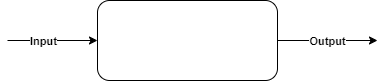
\includegraphics{figures/general_algorithm_diagram.png}
	\caption{Mô hình thuật toán chung, khối hình chữ nhật đen chưa định nghĩa gì, tượng trưng cho một chiếc hộp đen (blackbox). Hiểu rằng, thuật toán là biến đầu vào (Input) thành đầu ra (Output) tương ứng.}
	\label{fig:algorithm_architect_general}
\end{figure}

Như vậy khi tiến hành nêu ra định nghĩa thuật toán ở trên, ta nắm được một số thông tin mà sẽ được dùng để áp dụng kết nối chủ thể như "\textbf{hướng dẫn cho máy tính}", "\textbf{giải quyết vấn đề/bài toán}"



\section{Thuật toán trong góc nhìn sinh học}
Khi tìm hiểu về chủ thể này, sự thâm nhập của thuật toán vào lĩnh vực sinh học nói chung là cực kỳ thú vị. Trong mục này, bài viết xem thuật toán dưới góc nhìn di truyền nên những kiến thức có liên quan đến di truyền cũng sẽ được đề cập.

\subsubsection{Di truyền, ADN và nhiễm sắc thể}
Di truyền là hiện tượng truyền đạt các tính trạng của các (bố mẹ, tổ tiên) cho các thế hệ con cháu theo \cite{whatIsGenetic}.

ADN là phân tử mang thông tin di truyền quy định mọi hoạt động sống theo \cite{whatIsDNA}

Nhiễm sắc thể là bào quan chính chứa bộ gen của sinh vật, là cấu trúc quy định sự hình thành protein, có vai trò quyết định trong di truyền theo \cite{whatIsChronosome}. Có thể hiểu nhiễm sắc thể (NST) là một tập hợp của các gen.

Như vậy, mối quan hệ giữa các khái niệm có thể được mô tả theo sơ đồ sau:
\begin{figure}[h]
	\centering
	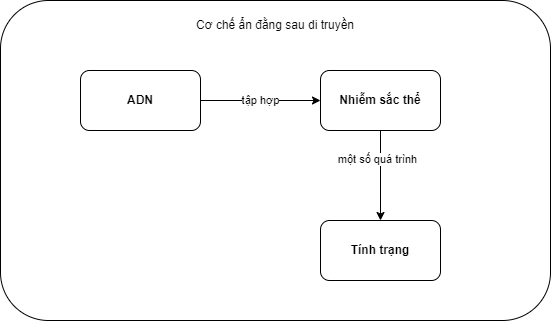
\includegraphics[scale=0.5, height=8cm]{figures/genetic_illustration_diagram.png}
	\caption{Sơ đồ mối quan hệ giữa các khái niệm. Về cơ bản ADN/NST qua một số giai đoạn trung gian để có thể biểu thị nên tính trạng. Và quá trình đó có thể hiểu là cơ chế biểu thị của di truyền}
	\label{fig:genetic_illustration_diagram}
\end{figure}

\noindent
Việc đề cập đến kiến thức di truyền nhằm khẳng định vai trò của di truyền là mang \textbf{tính hướng dẫn}. Điều này tương tự với nội dung đã đề cập trong định nghĩa của thuật toán \ref{sec:algorithm}.

Về bản chất của áp dụng trong mục này là nhận ra ADN/NST là có tính hướng dẫn tương tự như thuật toán. Sự suy luận này xuất phát từ việc đúc kết những đối tượng mang tính tương tự thường sẽ có một số tính chất chung.

Vậy câu hỏi mà mục này đặt ra là: "\textbf{Mình khai thác tính hướng dẫn mà sinh học nói chung mang lại cho thuật toán như thế nào?}"



\section{Tìm hiểu về thuật toán di truyền và trả lời câu hỏi trên}
Việc khai thác câu hỏi trên chính là việc cần đưa tính hướng dẫn đáp ứng tính chất thứ hai mà định nghĩa thuật toán (~\ref{sec:algorithm}) đã nêu. Đó là tính chất giải quyết vấn đề/bài toán.

Trong thực tế, nhiều thuật toán đã dựa trên các đối tượng sinh học để giải quyết yêu cầu đặt ra. Một trong số những thuật toán có thể kể đến như:
\begin{itemize}
	\item Thuật toán tối ưu đàn kiến (Ant Colony Optimization) \cite{AntColony}. Một thuật toán dựa trên hành vi tìm đường của quần thể kiến trong tự nhiên.
	
	\item Thuật toán tối ưu bầy hạt ((Particle Swarm Optimization) \cite{PSO}. Thuật toán cũng dựa trên hành vi di chuyển và tìm kiếm thức ăn của các đàn chim và đàn cá.
	
	\item Thuật toán sinh học miễn dịch (Artificial Immune System) \cite{AIS1} \cite{AIS2}. Một thuật toán lấy ý tưởng từ hệ thống miễn dịch của con người.
	
	\item và còn nhiều thuật toán khác nữa...
\end{itemize}

Về cơ bản, những dẫn chứng em cung cấp ở trên là một phần minh chứng cho câu hỏi lớn mà bài viết của em muốn khai thác. Tuy nhiên, hệ quả của câu hỏi đó mới là quan trọng. Ở mục này em xin bàn luận thêm sâu hơn về thuật toán di truyền xem như câu trả lời cho câu hỏi làm sao để áp dụng ý tưởng đó vào lập trình.

\subsection{Nền tảng Genetic Algorithm (GA)}
Thuật toán di truyền là một thuật toán lấy ý tưởng từ quá trình tiến hoá trong tự nhiên. Chính xác hơn, đây là thuật toán mô phỏng quá trình ấy và là một thuật toán tối ưu.

Quá trình tiến hoá trong tự nhiên còn hiểu là quá trình chọn lọc tự nhiên \cite{NaturalSelection}. Đây là quá trình mà những cá thể mang khả năng thích nghi (fitness) cao với môi trường sẽ có nhiều khả năng tồn tại và duy trì nòi giống để tạo ra thế hệ sau. Kết quả của quá trình này là qua nhiều thế hệ, thế hệ sau có khả năng cao sẽ mang những gen thích nghi tốt với môi trường.

Diễn giải thêm cho quá trình trên, \textbf{môi trường} và \textbf{di truyền} là hai yếu tố chi phối chủ đạo.

Phân tích thêm cho quá trình, ngoài hai yếu tố chi phối trên, quá trình này hoạt động trên một quần thể (một tập hợp các cá thể).

Như vậy, từ ý tưởng thô sơ là quá trình chọn lọc tự nhiên. Sau quá trình phân tích để xác định các yếu tố, bước tiếp theo là mình cần chuyển các yếu tố ấy thành mã lập trình dưới góc nhìn của \textbf{toán học}.

\subsection{Triển khai ở góc nhìn thuật toán}
Do bản chất của máy tính là tính toán nên mình phải cần nhìn vấn đề dưới góc nhìn của một người lập trình. Ở góc nhìn này, ta sẽ trả lời cho khía cạnh thứ hai của định nghĩa thuật toán (giải quyết vấn đề).

Máy tính còn mang tính tất định. Những yếu tố mô tả ở trên còn tương đối mơ hồ. Như vậy, sự rõ ràng của những khái niệm trên phải được xác lập. Dưới đây là những câu hỏi dùng để làm rõ thêm thuật toán di truyền.
\begin{itemize}
	\item Làm sao phản ánh được môi trường vào trong di truyền?
	\item Di truyền còn tương đối mơ hồ, làm sao để đảm bảo sự rõ ràng ở đây?
	\item Việc cài đặt quần thể là cài đặt như thế nào?
	\item Phản ánh giữa thuật toán và di truyền sẽ ra sao?
\end{itemize}

\subsection{Câu trả lời của thuật toán}
Trong GA, việc phản ánh môi trường vào trong di truyền được trả lời thông qua hàm fitness (hàm đánh giá độ thích nghi).

Ngoài phản ánh qua hàm fitness, môi trường còn phản ánh thông qua Selection. Selection hoạt động dựa trên giá trị thích nghi. Những cá thể có điểm thích nghi cao sẽ có khả năng giữ được phần gen của mình và truyền cho thế hệ sau. Selection còn có thể coi là một toán tử trong môi trường.

Di truyền ở mức độ chi tiết hơn ngoài \ref{fig:genetic_illustration_diagram} còn có thêm một số yếu tố sau để có thể triển khai thuật toán:
\begin{itemize}
	\item Lai ghép (Crossover). Hiểu là trao đổi thông tin di truyền ở giữa hai cá thể. Còn có thể hiểu thêm, việc tiến hành lai ghép là việc yêu cầu hai cá thể trong quần thể thực hiện sinh sản để cho ra cá thể con. Cá thể con sẽ mang một phần/toàn phần thông tin di truyền từ hai cá thể tổ tiên (có thể xem như cha và mẹ).
	\item  Đột biến (Mutation). Trong di truyền, quá trình đột biến xảy ra tương đối. Ở quá trình chọn lọc tự nhiên, đột biến đem đến sự đa dạng cho nguồn gen di truyền.
	\item  ADN/NST. Đây chính là mã di truyền. Đối với giải quyết vấn đề/bài toán thì ADN/NST chính là \textbf{lời giải tiềm năng}.  
\end{itemize}

Câu hỏi về cài đặt quần thể. Trong lập trình, điều này có thể được mô phỏng dưới dạng một tập hợp các mã di truyền. Ở góc độ lập trình, điều này đồng nghĩa với việc mình đang duy trì một tập lời giải.

Phản ánh giữa thuật toán và di truyền là mối quan hệ phản ánh đến từ việc nhìn các mã di truyền là lời giải cho vấn đề được nêu. Điều này dẫn đến hệ quả các phép toán như Crossover, Mutation sẽ đóng vai trò như việc trao đổi lời giải và đột ngột phát sinh ý tưởng mới.

\subsection{Mã giả thuật toán}
Qua những mục được đề cập trên, mã giả của thuật toán sẽ như sau:
\begin{algorithm}
	\caption{Thuật toán di truyền (GA)}
	\begin{algorithmic}[1]
		\State Khởi tạo quần thể $P$
		\State Đánh giá độ thích nghi cho từng cá thể trong $P$
		\While{Thoả điều kiện dừng} 
		\State Chọn cá thể trong $P$ dựa trên fitness
		\State Tiến hành lai ghép (Crossover) để tạo con cháu
		\State Thêm đột biến (Mutation)
		\State Tính thích nghi (dùng hàm Fitness) cho con cháu
		\State Chọn (Selection) thế hệ tiếp theo từ $P$ và con cháu
		\EndWhile
		\State Trả về cá thể tốt nhất
	\end{algorithmic}
\end{algorithm}

Thuật toán di truyền chỉ cố định ở mô hình thao tác (mã giả minh hoạ ở trên). Còn các chi tiết còn lại như hàm Fitness, cách chọn thế hệ, phương pháp lai ghép hay cách đột biến, chúng ta có thể hoàn toàn linh động. Tuỳ vào từng trường hợp mà sẽ dùng phương pháp khác nhau.

\noindent
Và ngoài ra, thuật toán di truyền cũng là một phần của lập trình tiến hoá (Evolution Programming) \cite{evolutionProgramming} cùng với một số thuật toán khác như Chiến lược tiến hoá (Evolution Strategy) \cite{EvolutionStrategy}, thuật toán di truyền vi phân (Differential Evolution) \cite{DifferientalEvolution1} \cite{DifferientalEvolution2}, ...

\par
Mục nội dung này được viết là dựa trên các nguồn \cite{GA1} \cite{GA2} \cite{GA3} \cite{GA4} \cite{GA5_Overview}


\section{Mạng Feedforward Neural Network (FNN) và mạng Artificial Neural Network (ANN)}
Tìm hiểu trên về thuật toán di truyền đã phần nào mở ra và chứng minh cho \hyperlink{main_question}{câu hỏi chủ đề} qua lĩnh vực sinh học. Ở mục này, câu hỏi sẽ tiếp tục được trả lời nhưng sẽ dưới góc nhìn của lĩnh vực triết học và khoa học thần kinh.

Mạng Feedforward Neural Network còn được hiểu là mạng lan truyền thẳng. Đây là một mạng lưới thần kinh nhân tạo. Để hiểu hơn về mạng này, hãy khảo sát sơ qua về lịch sử phát triển của AI thông qua tìm hiểu một số khuynh hướng phát triển của Deep Learning.

\subsection{Lịch sử phát triển của AI}
	Đây là phần nội dung được tổng hợp qua \cite[Chương 1, mục 1.2.1, trang 12--26]{Goodfellow-et-al-2016}
	
	AI mang trong mình một lịch sử phát triển dài hạn và qua nhiều khuynh hướng phát triển khác nhau. Những khuynh hướng phát triển ấy là kết quả của sự giao thoa nhiều lĩnh vực có thể kể đến như bio-learning (học tập lấy cảm hứng từ tự nhiên), cybernetic (điểu khiển học) và connectionism (hiểu là sự kết nối). 
	
	Những đóng góp khác nhau từ các lĩnh vực đã góp phần và làm tiền đề quan trọng cho sự nổi dậy của AI trong giai đoạn xã hội hiện nay. Và chính thực, ví như các mô hình ngôn ngữ lớn (Large Language Models) đều dựa trên những ý tưởng cốt lõi và thêm du nhập của sự chú ý (Attention \cite{vaswani2023attentionneed}).

\subsection{Ý nghĩa của AI trong bài viết này}
	Trong quá trình tìm tòi về Trí tuệ nhân tạo, em nhận ra tính kết nối và tổng hợp của nhiều lĩnh vực ở trong AI. Song song với điều đó, AI cũng là một thuật toán và do đó việc tiến hành ngâm cứu thêm về chủ thể này cũng sẽ góp phần trả lời cho câu hỏi chủ đề.
	
\subsection{Mối quan hệ giữa AI và thuật toán}
	Khẳng định AI là môt \textbf{biểu hiện của thuật toán}, là một khẳng định hợp lí. 
	
	Hãy xét đến đối tượng thực hiện định nghĩa tập hữu hạn các bước. Nếu lấy con người làm trung tâm đối chiếu thì sẽ phát sinh một số câu hỏi sau:
	\begin{itemize}
		\item Nếu đối tượng thực hiện định nghĩa là con người thì sao?
		\item Nếu đối tượng thực hiện không là con người?
	\end{itemize} 
	
	Tiến hành trả lời cho hai câu hỏi mang tính bổ trợ nhau ở trên, ta nhận ra AI là một dạng thuật toán nhưng việc thực hiện định nghĩa các bước giải quyết (tính hướng dẫn) phụ thuộc rất ít vào con người.

\subsection{AI, thuật toán và FNN}
	Khảo qua mối quan hệ kế thừa của các đối tượng như AI, thuật toán và FNN. Ta có sơ đồ sau:
	
	\begin{figure}[h]
		\centering
		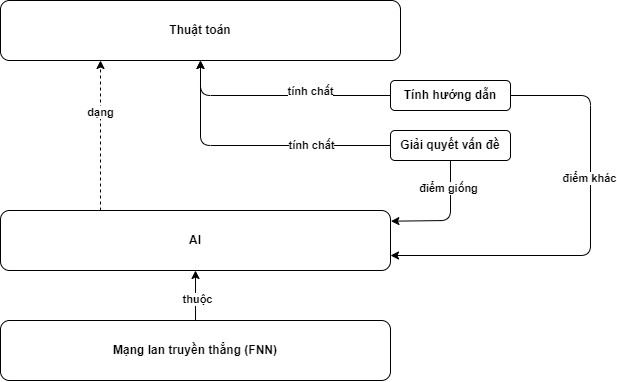
\includegraphics[scale=0.6]{figures/ai_fnn_algorithm.png}
		\caption{Mối quan hệ giữa AI, thuật toán và mạng lan truyền thẳng (FNN). AI giống thuật toán là đều dùng để giải quyết vấn đề nhưng khác nhau ở bước hướng dẫn. Mặt khác FNN là một con của AI, AI có những thuộc tính trên thì mạng FNN cũng sẽ có.}
		\label{fig:ai_fnn_algo_relationship}
	\end{figure}  
	
	Như vậy thông qua sơ đồ trên, ta biết được FNN sẽ có những tính chất mà AI có. Nhờ vậy, tìm hiểu thêm về mạng này cũng sẽ góp phần hiểu thêm về thuật toán.
	
\subsection{FNN}
	Để cho câu trả lời cho câu hỏi chủ đề được trọn vẹn. Hãy tìm hiểu sơ qua về mạng FNN.
	
	FNN là một cấu trúc cơ bản và quan trọng trong học sâu (Deep Learning). Dựa trên tiền đề này mà nhiều mạng với kiến trúc tiên tiến hơn được ra đời. Ngoài ra tính chất của FNN là thông tin chỉ lan truyền theo một chiều duy nhất xuyên suốt và không có vòng lặp.
	
	FNN là một dạng của mạng thần kinh nhân tạo (Artificial Neural Network). Tất có nghĩa, FNN là một tập hợp các neuron và sự kết nối giữa chúng.
	
	Mặt khác, do mang trong mình tính chất của một thuật toán nên để có thể diễn giải sang mã lập trình được thì cần thông qua một cây cầu mang tên \textbf{toán học}. Trong bối cảnh này, toán học dùng để mô phỏng hành vi của một đơn vị neuron và hành vi của một tập các neuron được kết nối với nhau. Về cụ thể:
	\begin{itemize}
		\item một đơn vị neuron có hành vi: nhận tín hiệu từ nhiều nguồn, tiến hành tổng hợp và đưa ra kết quả. Ở mặt này có thể dùng hàm số để mô phỏng hành vi. Cụ thể hơn, trong trường hợp này là hàm phi tuyến với công thức:
		
		\begin{equation}
			 f(x) = \sigma(w_0 + \sum_{i=1}^{n} w_{i} * x_{i})
		\end{equation}
		
		Hệ số $w_0$ là hệ số đền bù (bias) và $w_i$ là các trọng số kích hoạt ứng với đầu vào $x_i$, và $n$ là số lượng đầu vào.
		
		\item một tập hợp neuron. Mang hành vi kế thừa của các neuron nhưng sẽ nhận nhiều đầu vào và cho ra nhiều kết quả. Để làm được điều này, ma trận được dùng để mô phỏng hành vi. Ngoài ra việc dùng ma trận thay vì tập trung vào mô phỏng từng đơn vị sẽ đem đến hiệu quả tính toán tốt hơn.
		
		\begin{equation}
			f(X) = \sigma(W^TX + B)
		\end{equation}
		
		Với $X$ là một tập đầu vào với kích thước $ \text{data\_points} \times \text{input\_dim} $, $X$ là một ma trận. $W$ là tập trọng số với kích thước $ \text{output\_dim} \times \text{input\_dim} $. $W$ cũng là một ma trận và $W^T$ là ma trận chuyển vị. $B$ đóng vai trò như hệ số bù với kích thước $1 \times \text{output\_dim} $.
	\end{itemize}

	Ở mặt hình tượng, đây là sơ đồ của mạng FNN.
	
	\begin{figure}[h]
		\centering
		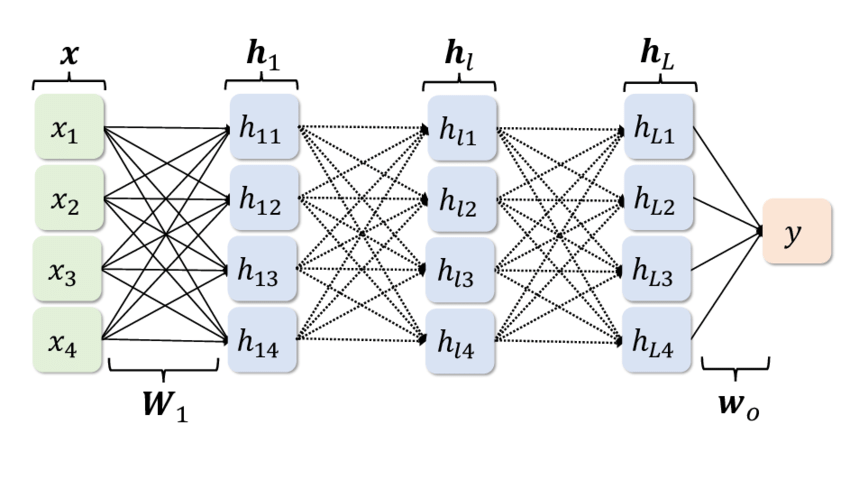
\includegraphics[scale=0.3]{figures/fnn.illustration.png}
		\caption{Ảnh minh hoạ cho mạng FNN \cite{fnn_figure}. Gồm các trọng số và các đơn vị. Mạng này có 5 tầng gồm 1 tầng đầu vào, 1 tầng đầu ra và 3 tầng ẩn.}
		\label{fig:fnn_illustration}
	\end{figure}
	
\noindent
Qua quá trình phân tích và tìm hiểu về mạng FNN, bài viết làm rõ thêm về mối quan hệ của các đối tượng. Qua đó khẳng định thêm về vị trí đứng của \textbf{toán học} trong câu hỏi \hyperlink{main_question}{"Người lập trình lấy ý tưởng từ đâu?"}

\section{Tính kết nối giữa GA và FNN}
\subsection{Ở phạm vi con người}
	Trước khi trả lời câu hỏi này, hãy khảo sát sơ qua ý tưởng ứng dụng thuật toán di truyền vào mạng Neural Network bằng cách đặt câu hỏi trong bối cảnh con người chúng ta.
	
	Không thể phủ nhận rằng, con người là một bản thể sinh học có sự sống, mỗi cá thể trong quần thể con người đều có những đặc điểm riêng đầy thú vị. Dựa trên lí giải sinh học, ta biết rằng chính gen là bộ khung tạo nên và làm cho quần thể con người tồn tại nhiều cá thể đầy thú vị.
	
	Và thú vị hơn nữa, mỗi chúng ta đều có một tư duy khác nhau và độc lập với người khác. Ở điểm này, vậy có phải di truyền cũng là thứ làm cho chúng ta khác biệt ở nhận thức? Đây là một câu hỏi mà để trả lời nó cần giao thoa quan điểm của nhiều thứ (di truyền, môi trường, xã hội, biến cố, …), song không thể gạt bỏ di truyền ra khỏi tư duy.
	
	Theo dòng chảy của suy luận trên, ta biết di truyền có kết nối với tư duy. Dựa trên mối kế thừa quan hệ ở lập trình, ta cũng phần nào đoán nhận giải thuật di truyền phải có một kết nối gì đó đến Neural Network.
	
	\begin{figure}[h]
		\centering
		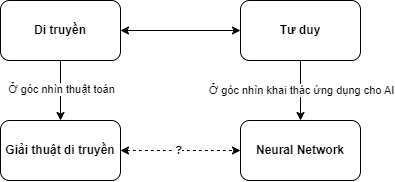
\includegraphics{figures/thought_and_genetic.png}
		\caption{Sơ đồ trên thể hiện Di truyền và tư duy có mối quan hệ với nhau. Thông qua góc nhìn thuật toán đối với di truyền làm phát sinh giải thuật di truyền, góc nhìn khai thác ứng dụng AI làm cho phát sinh mạng thần kinh nhân tạo (ANN). Mặt khác di truyền và tư duy có mối quan hệ, vậy thì giải thuật di truyền và ANN cũng phải có quan hệ tương tự. Dấu ? tượng trưng cho việc chưa xác định được mối quan hệ đó là gì.}
		\label{fig:thought_and_genetic}
	\end{figure}
	
\subsection{Thử khai thác dấu ?}
	Đặt mục tiêu khai thác trong bối cảnh mạng FNN, ta thấy FNN có một số điểm đáng lưu tâm như sau:
	\begin{itemize}
		\item Kiến trúc FNN. Đó là số lượng số đơn vị neuron, số tầng, hàm kích hoạt, số tham số.
		\item Tham số FNN. Là về các trọng số kết nối giữa các tầng. 
	\end{itemize}
	
	Mặt khác, một quy trình ứng dụng của mạng FNN gồm hai pha cơ bản sau:
	\begin{itemize}
		\item Pha đào tạo (Training). Là pha học của mạng. Là pha thay đổi các tham số sao cho việc chuyển đổi giữa X (Input) sang Y (Output) là tốt nhất có thể. \cite{kak1993training}
		\item Pha ứng dụng. Là pha khai thác mạng đã qua đào tạo, đem vào dùng với dữ liệu có thể chưa qua đào tạo.
	\end{itemize}
	
	Xét đến, thuật toán di truyền (Genetic Algorithm) là một thuật toán tối ưu. Tuân theo quy trình, ta nắm được GA sẽ tham gia vào pha đào tạo (Training). Xét đến những điểm đáng lưu tâm, ta khẳng định GA có thể dùng để tối ưu các thành phần của mô hình như kiến trúc và tham số. \cite{montana1989training}
	
\noindent

Đối với các mô hình AI hiện tại, thường việc tối ưu sẽ dựa trên các phương pháp liên quan đến Gradient. Thuật toán di truyền nói riêng và họ thuật toán tối ưu không dùng Gradient vẫn đang phát triển nhưng không nổi trội bằng nhánh trên.

\section{Ứng dụng GA, FNN vào tìm kiếm chiến lược sinh tồn của sinh vật}
\subsection{Mô tả vấn đề}
	Cho sự tồn tại của một môi trường với các thông số như nhiệt độ/độ ẩm/lượng thức ăn/mức năng lượng tối đa/ánh sáng/lượng mưa/độ Ph/tốc độ gió/số lượng kẻ thù.
	 
	Mỗi cá thể là một mạng Feedforward Neural Network với kiến trúc cố định (mô phỏng chiến lược sinh tồn). Mạng này nhận đầu vào là các thông số môi trường và trả kết quả đầu ra là chiến lược tìm kiếm thức ăn và cách phản ứng với kẻ thù.
	
	Hãy ứng dụng thuật toán di truyền nhằm tìm kiếm ra chiến lược sinh tồn phù hợp đối với môi trường được cho.

\subsection{Biện luận một số thành phần trong mô tả vấn đề}
	Chiến lược sinh tồn của sinh vật là cách mà sinh vật tương tác với môi trường. Ở đây, bài viết đặt bối cảnh trong sự tương tác với môi trường để biểu lộ cách mà thuật toán di truyền hoạt động cũng như gắn kết với quá trình chọn lọc tự nhiên.
	
	Việc chọn mạng FNN là dùng để mô tả thêm sâu cách mà sinh vật tương tác để cho ra chiến lược tối ưu.
	
	Sự chi phối của thuật toán di truyền đến mạng FNN là một ví dụ biểu thị cho mối quan hệ giữa GA và FNN, là cách di truyền ảnh hưởng đến tư duy.
	
\subsection{Ý tưởng triển khai}
	Trong vấn đề này, với kiến trúc mô hình là cố định, ta xác định yếu tố cần tối ưu là các tham số của mạng. Như vậy, hãy xem tập tham số tượng trưng như một cá thể. 
	
	Mỗi bước thực hiện tìm kiếm, ta duy trì một tập các quần thể như vậy. Qua một số thế hệ hoạt động, ta có được những cá thể tiềm năng (mang chiến lược sinh tồn hợp lí), đây là lời giải cho vấn đề được nêu.
	
	Hàm đánh giá độ thích nghi cá thể được thực thi qua các tiêu chí sau:
	\begin{itemize}
		\item Nếu chiến lược sinh tồn đưa ra mức năng lượng cao, khả năng nhận diện thức ăn tốt thì giá trị fitness cao (tăng cao khả năng tồn tại)
		\item Nếu môi trường có các điều kiện khắc nghiệt như mưa nhiều, áp suất thấp, độ Ph không ổn định thì fitness giảm
		\item Nếu chiến lược có khả năng chiến đấu tốt sẽ làm cho có lợi trong môi trường cạnh tranh (tuỳ vào môi trường)
	\end{itemize}
	
\subsection{Chi tiết một số thành phần thuật toán GA}
	Quần thể: là tập hợp các cá thể mang mã di truyền là các tham số của mạng FNN.
	
	Hàm Fitness: nhận đầu vào là cá thể và môi trường. Kết quả trả về sẽ là điểm đánh giá mức độ thích nghi của chiến lược. 
	\begin{equation}
		fitness = w_1 \times E + w_2 \times F - w_3 \times R - w_4 \times P - w_5 \times A + w_6 \times S
	\end{equation}
	Với $w_i$ là hệ số điểm đánh giá cho thành phần. $E$ là mức năng lượng tiêu thụ của sinh vật. $F$ là khả năng cảm nhận thức ăn của sinh vật. $R$ là RainFall (lượng mưa), giá trị được chuẩn hoá về khoảng 0,1. $P$ là ảnh hưởng của áp suất, giá trị cũng được chuẩn hoá về khoảng 0,1.
	$S$ là giá tri phản mức độ chiến đấu của sinh vật. Còn $A$ là phản kháng lại môi trường lí tưởng với công thức:
	\begin{equation}
	\text{A} =
	\frac{1}{5} \Bigg[
	\left( \frac{\text{Temp} - 25}{25} \right)^2 +
	\left( \frac{\text{Humid} - 50}{50} \right)^2 + \\
	\left( \frac{\text{Wind\_speed}}{200} \right)^2 +
	\left( \frac{\text{pH} - 7}{7} \right)^2 + \\
	\left( \frac{\text{Energy} - 5000}{10000} \right)^2
	\Bigg]
	\end{equation}
	
	Selection (Chọn lọc): được tiến hành dựa trên việc sắp xếp giá trị Fitness tương ứng với sinh vật. Số lượng cá thể bị loại đi sẽ chiếm một tỉ lệ cho trước so với tổng cá thể.
	
	Crossover (Lai ghép): được tiến hành hoàn toàn ngẫu nhiên trên những cá thể được giữ lại. Cách lai ghép đến từ việc lắp ghép các đoạn gen từ hai cha con. Cá thể mới được bổ sung thay thế cá thể bị loại bỏ mang id tương ứng.
	
	Mutation (Đột biến): được tiến hành hoàn toàn ngẫu nhiên trên tập quẩn thể. Chọn một cá thể, rồi chọn vị trí đột biến trên mã di truyền của cá thể. Rồi tiến hành đột biến.

\subsection{Kết quả thực thi thuật toán}
	Mã nguồn thuật toán được tham chiếu ở \cite{baolam}.
	
	Kết quả được chạy ở local với các thông số môi trường sau:
	\begin{figure}[h]
		\centering
		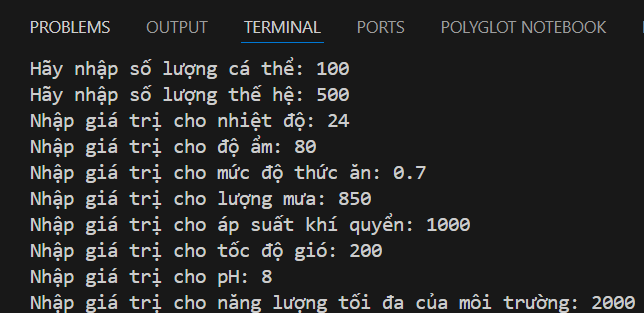
\includegraphics{figures/env_infor.png}
		\caption{Thông tin môi trường. Được nhập từ màn hình Console với thông tin được mô tả ở mục trên}
		\label{fig:env_infor}
	\end{figure}
	
	Với thông số trên, tiến hành đào tạo quần thể gồm 100 cá thể, qua 500 thế hệ, ta có kết quả:
	\begin{figure}[h]
		\centering
		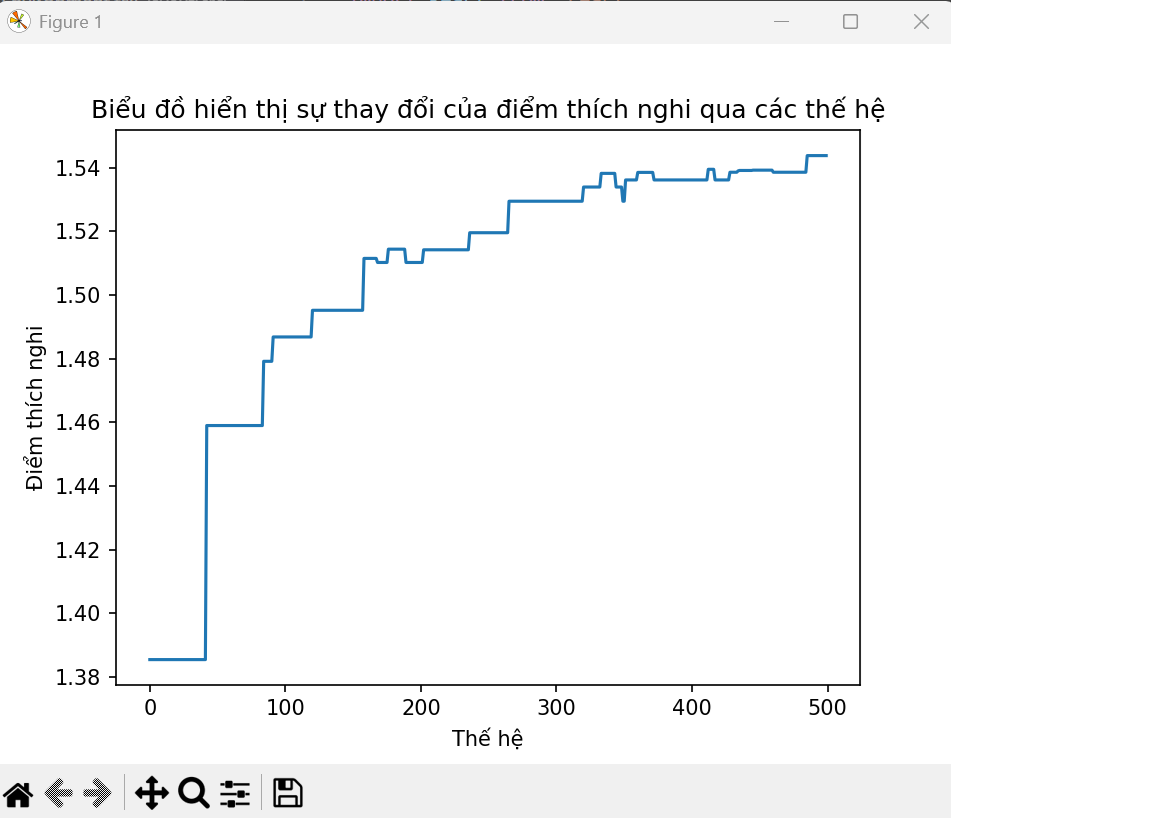
\includegraphics[scale=0.6]{figures/result.png}
		\caption{Biểu đồ ghi nhận giá trị Fitness cao nhất qua các thể hệ. Tuy có những thế hệ mà điểm Fitness tăng rùi lại giảm (do tác động của tính ngẫu nhiên) nhưng xu hướng chung là tăng theo thời gian.}
		\label{fig:result}
	\end{figure}
	
	Thực thi trên mã nguồn, sẽ hiển thị được thêm một số kết quả khác như thông số cài đặt thuật toán, mối quan hệ tổ tiên của một cá thể, ...
 	
\section{Kết luận}
	Thông qua phân tích và trả lời câu hỏi, bài viết đem đến một góc nhìn rõ ràng hơn về vai trò của người lập trình, quy trình tiếp thu và xử lý ý tưởng cũng như thiết lập vai trò của toán học trong lập trình.
	
	Bài viết triển khai từ những ý tưởng chung nhất đến ý tưởng riêng và cô lập hơn. Mẫu hình triển khai này có thể được dùng cho việc tìm lời giải cho vấn đề.
	
	Ngoài ra, qua quá trình phân tích, bài viết đi đến kết luận là AI cũng là một dạng thuật toán nên với vai trò là một người lập trình, chúng ta nên khai thác AI hiệu quả hơn nữa.
 	
 	Bài viết tập trung nhiều vào việc chứng minh câu hỏi chủ đề và xác lập những hệ quả có ý nghĩa của câu hỏi đó nên những nội dung được cập sẽ có những mục chưa đủ độ sâu nên bài viết dùng thêm phần Tài liệu để mở rộng thêm.
 
\section{Tham khảo thêm}
\printbibliography

\section{Minh hoạ bổ sung}
\begin{algorithm}
	\caption{Lai ghép giữa các sinh vật được giữ lại}
	\begin{algorithmic}[1]
		\Require Danh sách sinh vật được giữ lại $kept\_creatures$, độ dài ADN $adn\_length$, chỉ số bị loại $removed\_idx$, thế hệ hiện tại $generation$
		\Ensure Sinh vật con mới được tạo từ phép lai ghép
		\State Chọn ngẫu nhiên $parent1$ từ $kept\_creatures$
		\State Chọn ngẫu nhiên $parent2$ từ $kept\_creatures$
		\State $k \gets$ Số nguyên ngẫu nhiên trong khoảng $[0, adn\_length - 1]$
		\State $adn \gets parent1.adn()[0:k] + parent2.adn()[k:adn\_length]$
		\State Tạo sinh vật con $child$ với ID $removed\_idx$, thế hệ $generation + 1$, ADN $adn$
		\State Thêm $parent1.id$ vào danh sách tổ tiên của $child$
		\State Thêm $parent2.id$ vào danh sách tổ tiên của $child$
		\State \Return $child$
	\end{algorithmic}
\end{algorithm}

\begin{algorithm}
	\caption{Đột biến quần thể sinh vật}
	\begin{algorithmic}[1]
		\Require Danh sách sinh vật $creatures$, tỷ lệ đột biến $mutation\_rate$, độ dài ADN $adn\_length$
		\Ensure Quần thể sinh vật sau khi đột biến
		\State $population \gets$ độ dài của $creatures$
		\State $mutated\_length \gets mutation\_rate \times population$
		\State $mutated\_creatures \gets$ Chọn ngẫu nhiên $mutated\_length$ sinh vật từ $creatures$
		\For{\textbf{each} $creature$ \textbf{in} $mutated\_creatures$}
		\State $gene\_index \gets$ Số nguyên ngẫu nhiên trong khoảng $[0, adn\_length - 1]$
		\State $value \gets$ Số thực ngẫu nhiên trong khoảng $[-1, 1]$
		\State $adn \gets creature.adn()$
		\State $adn[gene\_index] \gets value$
		\State $creature.update\_adn(adn)$
		\State $creature.mutated\_position.append(gene\_index)$
		\EndFor
		\State \Return $creatures$
	\end{algorithmic}
\end{algorithm}

\begin{figure}[h]
	\centering
	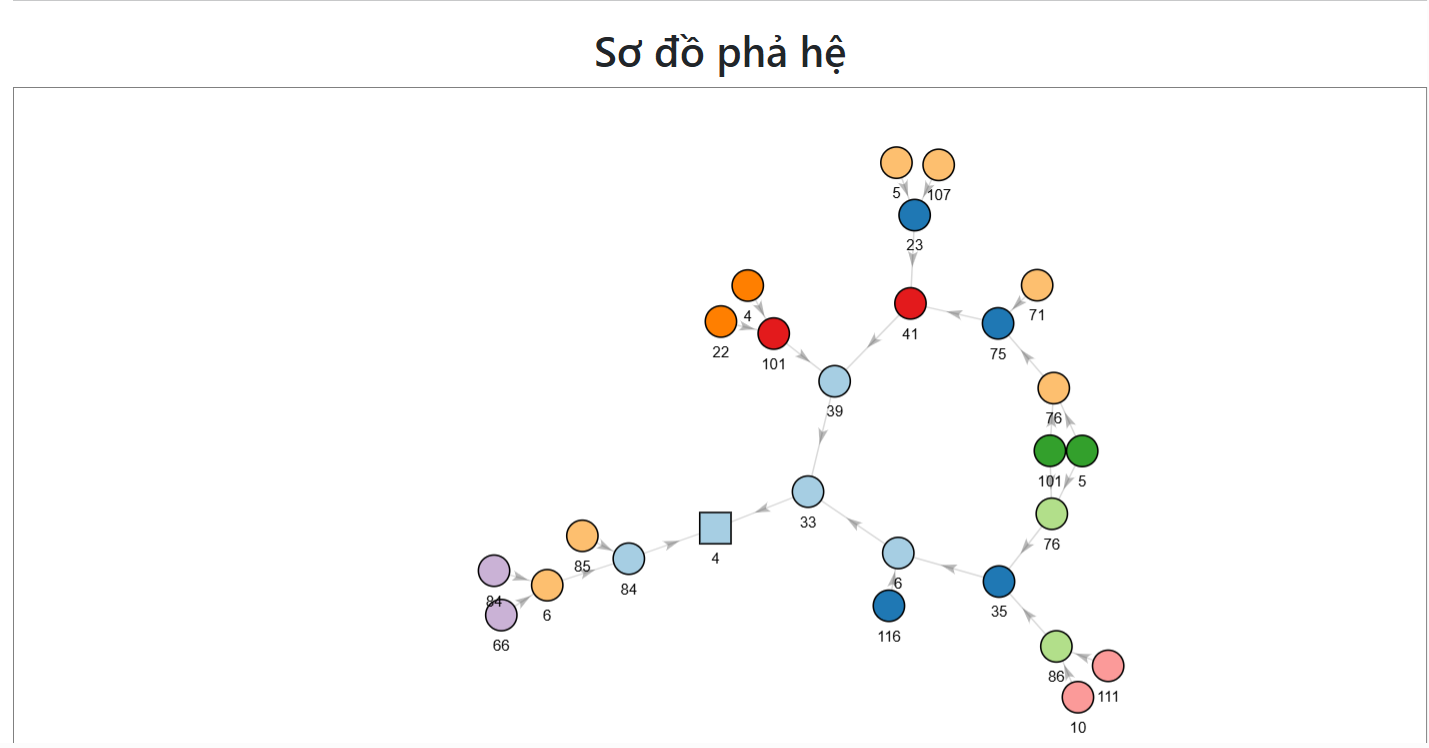
\includegraphics[scale=0.5]{figures/creature_relationship.png}
	\caption{Sơ đồ thế hệ kế thừa của một cá thể. Hình vuông thể hiện cá thể mục tiêu, mã màu khác nhau biểu thị cho thế hệ. Con số ghi dưới mỗi hình tượng trưng cho Id của cá thể.}
\end{figure}


\end{document}          
